\section{Data-Driven Curation Methodology}
\label{sec:methodology}

Most paper surveys are static artifacts: the authors manually curate a list, write the manuscript, and the list rapidly goes out of date. Reproducing or extending such surveys requires re-doing the curation from scratch, a labor-intensive and error-prone process. Our approach treats the paper list itself as a living, structured dataset---a design choice that supports automated validation, continuous updates, and reproducible scholarship.

\subsection{Single Source of Truth}

All paper metadata is stored in \texttt{papers.yaml} in the repository root. Each entry includes title, date (YYYY-MM), URL, taxonomy category (factual, experiential, or working), subcategory (token-level, parametric, or latent), authors, venue, code URL, project URL, abstract, and tags. The YAML format was chosen because it is human-readable, diffable, and easy to version-control. As of June 2026, \texttt{papers.yaml} contains 220 entries spanning from 2013 to 2026.

This single file drives all downstream outputs through a deterministic generation pipeline.

\subsection{Pipeline Overview}

Figure~\ref{fig:pipeline} illustrates the full data pipeline, which proceeds through five stages:

\begin{enumerate}
  \item \textbf{Extraction.} The generator reads \texttt{papers.yaml} and normalizes all fields. Each paper is assigned a stable identifier derived from its URL.
  \item \textbf{Validation.} An automated validator checks every entry for structural correctness: required fields are non-empty, URLs follow a whitelist of allowed domains (arXiv, ACL Anthology, OpenReview, DOI), date formats are valid, category--subcategory pairs are legal (e.g., ``working/parametric'' is a valid cell), and no duplicate URLs exist.
  \item \textbf{README generation.} The generator produces the Markdown document displayed on GitHub, grouping papers by category and subcategory and chronologically within each group.
  \item \textbf{JSON export.} A JSON version of the paper list is written to \texttt{docs/papers.json}, which powers an interactive web interface with client-side filtering by category, subcategory, date range, and keyword search.
  \item \textbf{BibTeX export.} The generator produces \texttt{paper/references.bib} for use in LaTeX compilation.
\end{enumerate}

The generator is fully idempotent: running it twice on the same input produces identical output. A \texttt{--check} flag runs validation and generation without writing any files, enabling use in CI pipelines.

\subsection{Automation Scripts}

Three Python scripts implement the pipeline:

\texttt{validate\_papers.py} performs comprehensive structural and semantic validation. It checks that all URLs are reachable (or at least well-formed), normalizes arXiv URLs to a canonical form (e.g., ensuring \texttt{abs/} paths), detects potential duplicates by comparing normalized titles and URLs, and verifies that category--subcategory assignments follow the taxonomy's allowlist. It is designed to run on every pull request.

\texttt{fetch\_metadata.py} enriches \texttt{papers.yaml} by querying arXiv's OAI-PMH API and Semantic Scholar for missing fields: author lists, publication venue, abstract text, and DOI. It respects rate limits and caches results locally to avoid redundant queries. This script is run periodically to fill in entries that were added with minimal metadata.

\texttt{fetch\_new\_papers.py} implements arXiv-based discovery. Given a date range and a set of search keywords (e.g., ``agent memory,'' ``episodic memory,'' ``long-term memory''), it queries the arXiv API for new submissions, filters by relevance to agent memory, and outputs candidate entries for human review. This reduces the manual effort of staying current: the script surfaces candidates, and the curator accepts, rejects, or modifies each one.

\subsection{Continuous Integration}

A GitHub Actions workflow (\texttt{.github/workflows/validate.yml}) runs \texttt{validate\_papers.py} with the \texttt{--check} flag on every pull request and on every push to the main branch. The workflow fails if any validation error is found---duplicate URL, malformed entry, or invalid category. This ensures that the paper list remains internally consistent even as multiple contributors submit changes. A CONTRIBUTING.md file provides contributor guidelines, and issue and pull request templates standardize submissions.

\subsection{Web Interface}

The JSON export (\texttt{docs/papers.json}) is consumed by an HTML page at \texttt{docs/index.html}, deployed via GitHub Pages at \url{https://tobias-weiss-ai-xr.github.io/agent-memory-research/}. The interface provides client-side filtering without any server-side infrastructure: users can search by keyword, filter by taxonomy cell, sort by date, and copy formatted citations. This makes the paper list accessible to researchers who prefer browsing over reading a static list.

\subsection{Reproducibility and Generalizability}

The entire pipeline---CIs, scripts, data file, and documentation---resides in a single open-source repository licensed under MIT. The \texttt{--check} flag enables anyone to verify that the paper list is valid without modifying any files. Because the pipeline is language-agnostic and domain-agnostic, it can be adapted to any living survey in any field: replace \texttt{papers.yaml} with domain-specific entries, adjust the validation rules, and deploy the web interface. We believe this methodology offers a template for community-maintained, data-driven surveys that remain current beyond a single publication date.

\begin{figure}[ht]
    \centering
    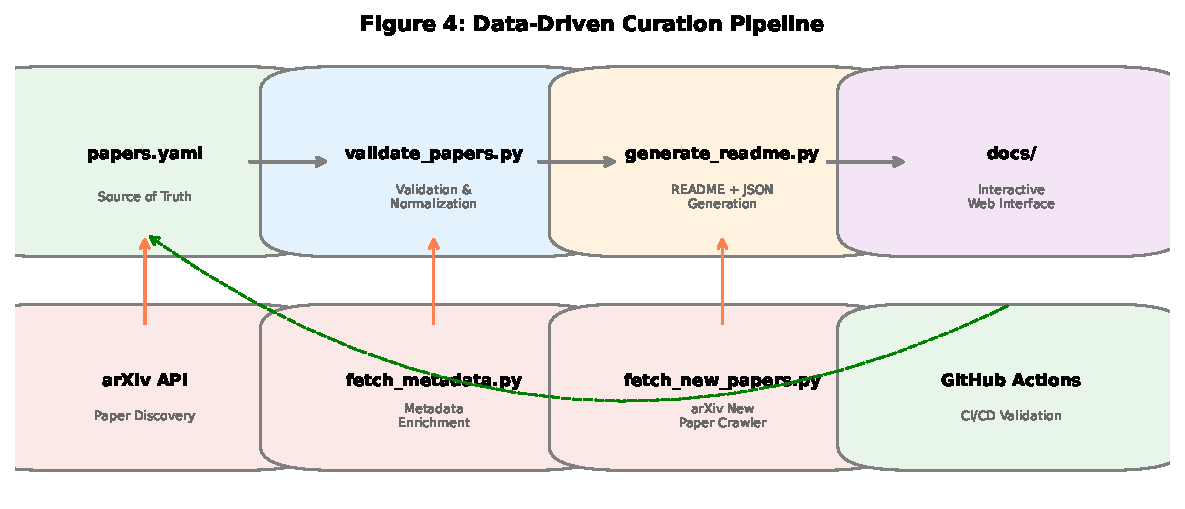
\includegraphics[width=\textwidth]{figures/fig4_pipeline.pdf}
    \caption{Data curation pipeline: from arXiv discovery through validation and publication.}
    \label{fig:pipeline}
\end{figure}
